\section{Spannung im Boden}
\begin{minipage}[t]{0.25\linewidth}
		$\rightarrow$ TR auf RAD!
		\vspace{\baselineskip} \\
		\begin{tabular}{ll}
		$\Delta \sigma_z=q \cdot J(a,b,z)$	& $\rightarrow a<b$ \\
											& $\rightarrow z=$Tiefe \\
											& $\rightarrow q=$Belastung $\left[\frac{kN}{m^2}\right]$ \\
											& $\rightarrow J=$Tab. s. 6.10f \\
											& $\rightarrow J=\frac{1}{2\cdot \pi} \cdot \left[arctan(\frac{a \cdot b}{R \cdot z}) + \frac{a \cdot b \cdot z}{R} \cdot  \left(\frac{1}{a^2 + z^2} + \frac{1}{b^2 + z^2}\right) \right]$ \\
											& $\rightarrow R^2=a^2 + b^2 + z^2$ \\	
		\end{tabular}

 % \textbf{vertikal Schnitt \& a,b-Feld} \\
 	\vspace{\baselineskip}
 \end{minipage}
 \begin{minipage}[t]{0.3\linewidth}
	\vspace{\baselineskip}
	\qquad 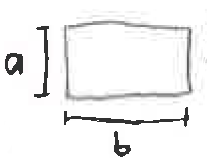
\includegraphics[width=0.3\linewidth]{images/SpimBoden1.PNG}
 \end{minipage}
\begin{minipage}[t]{0.5\linewidth}
		\medskip
		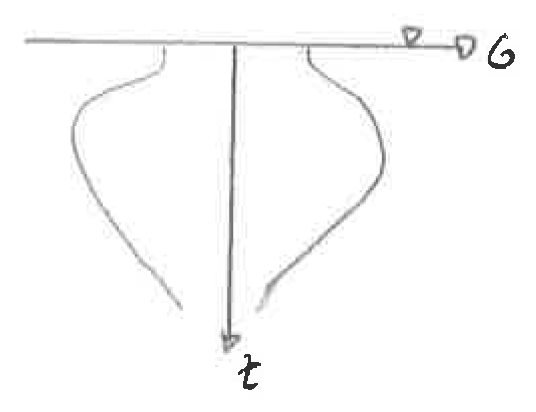
\includegraphics[width=0.5\linewidth]{images/SpimBoden2Verlauf.PNG}
\end{minipage}
 	

\begin{minipage}{0.7\linewidth}
	\begin{tabular}{|l|l|l|l|l|l|l|l|}
		\hline
		Schicht	& $\Delta$ z	& z$_m$		& $\sigma`_zm$	& J$_{a/b/c}$	& $\Delta \sigma_{a/b/c}$ 	& $\varepsilon_{a/b/c}$ 	& $\Delta$s \\
		& [m]			& [m]		&  [kPa]		& 				& $\left[\frac{kN}{m^2}\right]$ &		& [m] \\ \hline
		
		&		& \multicolumn{2}{c|}{$\cdot (\gamma - \gamma_w)$} &		\multicolumn{2}{c|}{$\cdot q_{Auflast}$} & \multicolumn{2}{c|}{$\qquad \cdot \Delta z$} \\
		&	&	&	&	& \multicolumn{2}{c|}{$\frac{1}{E}$} & \\
		%next Line
		&	&	&	&	&\multicolumn{2}{c|}{ od. $\varepsilon=\frac{C_c}{1 + e_0} \cdot log \frac{\sigma`_z + \Delta \sigma}{\sigma`_z}$} & \\ \hline 	
	\end{tabular}
	\vspace{\baselineskip}
\end{minipage}	
\begin{minipage}{0.4\linewidth}
		\begin{tabular}{l|l|l|l}
			\hline
			z	&	$\frac{z}{R}$	&	$\frac{a}{R}$ (J)	&	J$_{def/int}$	\\ \hline
				& \qquad	t		&	J$_t$				&	\\
				&	x				&						& $J_t - (J_t - J_h) \cdot \frac{x - t}{h - t}$	\\
				& \qquad	h		&	J$_h$				&	\\
		\end{tabular}
		\vspace{\baselineskip} \\
\end{minipage}



	\begin{minipage}{\linewidth}
	\begin{tabular}{|l|l|l|l|l|l|l|l|l|l|l|}
		\hline
		Schicht	& $\Delta$ z	& z$_m$		& $\sigma`_zm$	& J$_{a/b/c}$	& $\Delta \sigma_{a/b/c...w}$ 	& $\varepsilon_{a/b/c...w}$ 	& $\Delta s_w$ & $\Delta \sigma_E$ & $\varepsilon_E$ & $\Delta s_E$	\\
		%nxt Line
		& [m]			& [m]		&  [kPa]		& 				& $\left[\frac{kN}{m^2}\right]$ &		& [m] 	& $\left[\frac{kN}{m^2}\right]$ &		 & $\left[\frac{kN}{m^2}\right]$ \\ \hline
		\multicolumn{11}{|c|}{$\rightarrow$ $\Delta s = \Delta s_w + \Delta s_E$} \\
	\end{tabular}
	
	\vspace{\baselineskip}
	\end{minipage}


\begin{minipage}{0.5\linewidth}
	$\rightarrow$ \textbf{linear}: \\
	$\Delta \sigma_w=$ Wiederbelastung $=z \cdot \gamma$ [kPa] \\
	$\Delta \sigma_E=$ Bodenpressung $=q - \sigma_w$ [kPa] \\
	q $=$ Zusatzbelastung \\
	$\varepsilon_w = \frac{\Delta \sigma_w}{M`_E}$ ; $\varepsilon_E = \frac{\Delta \sigma_E}{M_E}$ \\
	$\Delta s_w = \Delta z \cdot\varepsilon_w$ ; $\Delta s_E = \Delta z \cdot\varepsilon_E$\\
\end{minipage}	
\begin{minipage}{0.5\linewidth}
	$\rightarrow$ \textbf{logarithmisch} analog linear jedoch: \\
	$\varepsilon_w = \frac{c_s}{1 + e_0} \cdot log \frac{\sigma`_z + \Delta \sigma_w}{\sigma`_z}$ wobei $\sigma`_z =$ 100 kPa \\
	$\varepsilon_E = \frac{c_c}{1 + e_0} \cdot log \frac{\sigma`_z + \Delta \sigma_w + \Delta \sigma_E}{\sigma`_z + \Delta \sigma_w}$ wobei $\sigma`_z =$ 100 kPa \\
	$\Delta s_w= \varepsilon_w \cdot \Delta z$ ; $\Delta s_E= \varepsilon_E \cdot \Delta z$ \\
		\vspace{\baselineskip}
\end{minipage}


\begin{minipage}{0.2\linewidth}
%		\vspace{\baselineskip}
	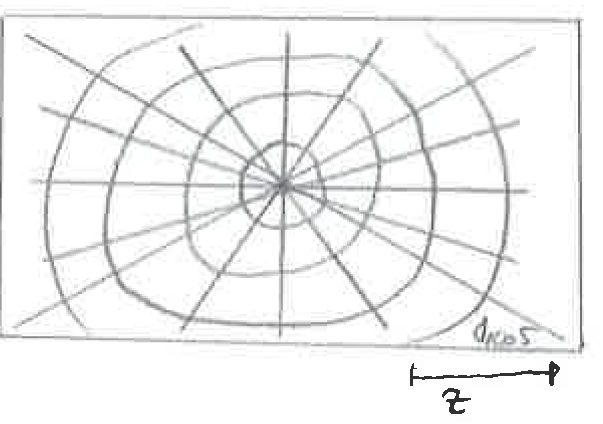
\includegraphics[width=\linewidth]{images/SpimBoden3Newmark.PNG}
\end{minipage}
\begin{minipage}{0.5\linewidth}
	\medskip
		\textbf{Newmark-Verfahren} $_{Bsp. S. 6.14}$ \\
		$\rightarrow$ belasteter Pkt in Mitte \\ 
		$\rightarrow$ Felder Zählen \\
		$\rightarrow$ $\sigma_z=q \cdot n \cdot 0.005$ \\
		$\rightarrow$ Massstab: $\frac{x}{z} = \frac{cm}{1m}$ \\
\end{minipage}




%	\begin{minipage}{\linewidth}
%		\vspace{\baselineskip}
%		\begin{tabular}{ll}
%		\textbf{Newmark-Verfahren} $_{Bsp. S. 6.14}$ & $\rightarrow$ belasteter Pkt in Mitte \\ 
%										 & $\rightarrow$ Felder Zählen \\
%										 & $\rightarrow$ $\sigma_z=q \cdot n \cdot 0.005$ \\
%		\end{tabular}
%		
%	
%	\end{minipage}
